\documentclass{article}
\usepackage[letterpaper, portrait, margin=1in]{geometry}
\usepackage{float}
\usepackage{graphicx}
\usepackage{listings}
\usepackage[]{indentfirst}
\usepackage{setspace}
\usepackage{amsmath}
\usepackage{amssymb}
\usepackage{mathtools}
\usepackage{esint}
\doublespacing

\begin{document}

\begin{center}
\LARGE{Task 5 Theory}
\end{center}
\mbox{}

Our half annulus can be defined as the region where $\frac{1}{2}\leq r\leq 1$ and $0\leq\pi\leq 1$, plotted below:
\begin{figure}[H]
	\centering
	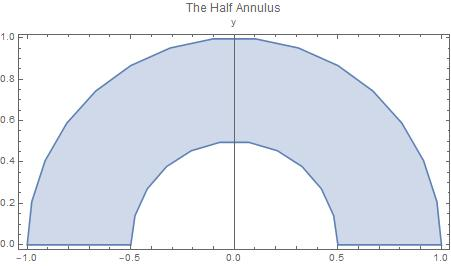
\includegraphics[width=4in]{HPC_HW_5_Annulus}
\end{figure}
Green's Theorem states that for most functions P(x,y) and Q(x,y):
\begin{equation*}
\iint_{D}(\frac{\partial Q}{\partial x}-\frac{\partial P}{\partial y})dA=\oint_{C}Pdx+Qdy
\end{equation*}
D is the region being integrated over and C is the positively oriented (counterclockwise) boundary of D.\\
To compute the area of D, we usually integrate the function f(x,y)=1 over the region. However, we can also use Green's Theorem to compute area by choosing P and Q such that $\frac{\partial Q}{\partial x}-\frac{\partial P}{\partial y}=1$. Any P and Q that satisfy this work and the area is equal to resulting line integral $\oint_{C}Pdx+Qdy$. For this problem, it is simplest to set P=0 and Q=x. This leaves us with the formula:
\begin{equation*}
A=\oint_{C}x\space dy
\end{equation*}
The boundary of the annulus can be broken into 4 parts and parameterized as follows for $t_i\epsilon[0,1]$:\\
\begin{center}
	\begin{tabular}{|c|c|c|c|c|}
    	\hline
		i & $x(t_i)$ & $y(t_i)$ & $\frac{dy_i}{dt}$ & $\vec{n}$ \\
        \hline
        1 & $cos(\pi t)$ & $sin(\pi t)$ & $\pi cos(\pi t)$ & $\cos(\pi t)\hat{x}+sin(\pi t)\hat{y}$ \\
        \hline
        2 & $\frac{t}{2}-1$ & 0 & 0 & $-\hat{y}$ \\
        \hline
        3 & $-\frac{1}{2}cos(\pi t)$ & $\frac{1}{2}sin(\pi t)$ & $\frac{\pi}{2} cos(\pi t)$ & $cos(\pi t)\hat{x}-sin(\pi t)\hat{y}$ \\
        \hline
        4 & $\frac{t}{2}+\frac{1}{2}$ & 0 & 0 & $\hat{y}$ \\
        \hline
    \end{tabular}
\end{center}
\mbox{}\\
Curve 1 is the outer semicircle (oriented counterclockwise), curves 2 and 4 are the left and right edges along the x-axis, and curve 3 is the inner circle (oriented clockwise). When followed in order, they combine to make the boundary of the half annulus. Then our area $A=\oint_{C}xdy=\int_{0}^{1}\sum_{i=1}^{4}x_i(t)dy_i(t)dt$\\ $=\int_{0}^{1}cos(\pi t)\cdot(\pi cos(\pi t))+0\cdot(\frac{t}{2}-1)-\frac{1}{2}cos(\pi t)\cdot(\frac{\pi}{2} cos(\pi t))+0\cdot(\frac{t}{2}+\frac{1}{2})\mbox{ }dt=\int_{0}^{1}(\pi-\frac{\pi}{4})\cdot cos^2(\pi t)dt$\\ $=\frac{3\pi}{4}[\frac{x}{2}-\frac{sin(2\pi x)}{4\pi}]_0^1=\frac{3\pi}{4}\cdot(\frac{1}{2}-0)=\underline{\frac{3\pi}{8}\approx1.1781}$.\\
If we compute the area directly using the formula for the area of a half annulus (derived from the area of a circle), we get $A=\frac{\pi}{2}\cdot(1^2-0.5^2)=\frac{\pi}{2}\cdot\frac{3}{4}=\underline{\frac{3\pi}{8}}$. Therefore Green's Theorem works well for this example. For a general area, one can numerically compute and differentiate x and y then apply Green's Theorem. The unit normal vectors ($\vec{n}$) are also tabulated in closed form above and can generally be computed numerically, though they could be extremely inaccurate along a complicated boundary.
\end{document}